\documentclass[12pt,a4paper,final]{article}
\usepackage[left=2.5cm,right=2.5cm,top=2.5cm,bottom=2.5cm]{geometry}

%% IDIOMA
\usepackage[utf8]{inputenc}
\usepackage[portuguese]{babel}

%% TRANSFORMAÇÕES ESTILO CSS
\usepackage{graphicx}

%% ESTÉTICA
\usepackage{enumerate}
\usepackage{booktabs}
\usepackage{amsmath, amsthm, amssymb, amsfonts}
\usepackage{multirow}
\usepackage[hyphens]{url}
\usepackage{subfig}

%% FONTE
\usepackage[T1]{fontenc}
%\usepackage[sc]{mathpazo} % Palatino with smallcaps
\usepackage{mathptmx}
\usepackage{eulervm} % Euler math

%% TIPOGRAFIA
\usepackage{parskip}
\usepackage[activate={true,nocompatibility},final,tracking=true,kerning=true,spacing=true,factor=1100,stretch=10,shrink=10]{microtype}

%% CODIGO
\usepackage{listings}
\usepackage{color}

\definecolor{dkgreen}{rgb}{0,0.6,0}
\definecolor{gray}{rgb}{0.5,0.5,0.5}
\definecolor{mauve}{rgb}{0.58,0,0.82}

\lstset{frame=tb,
  aboveskip=3mm,
  belowskip=3mm,
  showstringspaces=false,
  columns=flexible,
  basicstyle={\small\ttfamily},
  numbers=none,
  numberstyle=\tiny\color{gray},
  keywordstyle=\color{blue},
  commentstyle=\color{dkgreen},
  stringstyle=\color{mauve},
  breaklines=true,
  breakatwhitespace=true,
  tabsize=3
}

\title{Relatório 8 de TCC2/IC}
\author{Ly Sandro Amorim de Campos Salles\\Departamento de Física\\Universidade Federal do Paraná}
\date{\today}

\begin{document}
	\maketitle

  Desde o último encontro foram realizadas as seguintes atividades:

  Obtenção de cinco conjunto de dados, com 20000 pontos cada, para $L=250$ e $q\in\{$ 
  $0.1,$ $0.2,$ $0.3,$ $0.4,$ $0.5,$ $0.6,$ $0.7,$ $0.8,$ $0.9,$
  $1,$ $1.2,$ $1.4,$ $1.6,$ $1.8,$ 
  $2,$ $2.2,$ $2.4,$ $2.6,$ $2.8,$ 
  $3,$ $3.2,$ $3.4,$ $3.6,$ $3.8,$
  $4,$ $4.2,$ $4.4,$ $4.6,$ $4.8,$
  $5,$ $5.2,$ $5.4,$ $5.6,$ $5.8,$
  $6,$ $6.2,$ $6.4,$ $6.6,$ $6.8,$
  $7,$ $7.2,$ $7.4,$ $7.6,$ $7.8,$
  $8,$ $8.2,$ $8.4,$ $8.6,$ $8.8,$
  $9,$ $9.2,$ $9.4,$ $9.6,$ $9.8,$ $10,$
  $11,$ $12,$ $13,$ $14,$ $15,$ $16,$ $17,$ $18,$ $19,$ $20,$
  $22,$ $24,$ $26,$ $28,$ $30,$ $32,$ $34,$ $36,$ $38,$ $40,$
  $42,$ $44,$ $46,$ $48,$ $50,$ $52,$ $54,$ $56,$ $58,$ $60,$
  $65,$ $70,$ $75,$ $80,$ $85,$ $90,$ $95,$ $100,$ $110,$
  $120,$ $130,$ $140,$ $150,$ $160,$ $170,$ $180,$ $190,$
  $200,$ $220,$ $240,$ $260,$ $280,$ $300,$ $320,$ $340,$ $360,$ $380,$
  $400,$ $420,$ $440,$ $460,$ $480,$ $500,$ $520,$ $540,$ $560,$ $580,$
  $600,$ $620,$ $640,$ $660,$ $680,$ $700,$ $720,$ $740,$ $760,$ $780,$
  $800,$ $820,$ $840,$ $860,$ $880,$ $900,$ $920,$ $940,$ $960,$ $980,$
  $1000\}$. O gráfico obtido para a afinidade está na Figura \ref{fig:L250}.

  \begin{figure}[h]
    \centering
    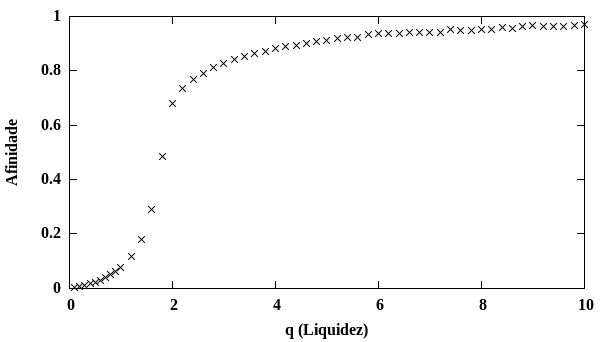
\includegraphics[width=.7\linewidth]{L250.png}
    \caption{Afinidade em função da liquidez para $L = 250$. A curva é uma sigmóide com uma inclinação no ponto crítico maior do que as observadas para $L=50$ e $L=100$.}
    \label{fig:L250}
  \end{figure}
  

  Obtenção de cinco conjunto de dados, com 10000 pontos cada, para $L=500$ e $q\in\{$
  $0.2,$ $0.4,$ $0.6,$ $0.8,$ $1,$
  $1.2,$ $1.4,$ $1.6,$ $1.8,$	$2,$
  $2.2,$ $2.4,$ $2.6,$ $2.8,$ $3,$
  $3.2,$ $3.4,$ $3.6,$ $3.8,$ $4,$
  $4.2,$ $4.4,$ $4.6,$ $4.8,$ $5,$
  $5.2,$ $5.4,$ $5.6,$ $5.8,$ $6,$
  $6.2,$ $6.4,$ $6.6,$ $6.8,$ $7,$
  $7.2,$ $7.4,$ $7.6,$ $7.8,$ $8,$
  $8.2,$ $8.4,$ $8.6,$ $8.8,$ $9,$
  $9.2,$ $9.4,$ $9.6,$ $9.8,$ $10$
  $\}$. Não foi possível obter os datos de afinidade para este conjunto de dados pois o software de regressão linear utilizado não conseguiu processar os grandes valores gerados pela simulação. 

  Foram obtidos os gráficos das derivadas para a afinidade em função da Liquidez $q$. Foi comprovado o aumento da inclinação no ponto crítico para os gráficos de Afinidade versus Liquidez. Esses resultados estão nas Figuras \ref{fig:L50-derivada}, \ref{fig:L100-derivada} e \ref{fig:L250-derivada}.

  \begin{figure}[h]
    \centering
    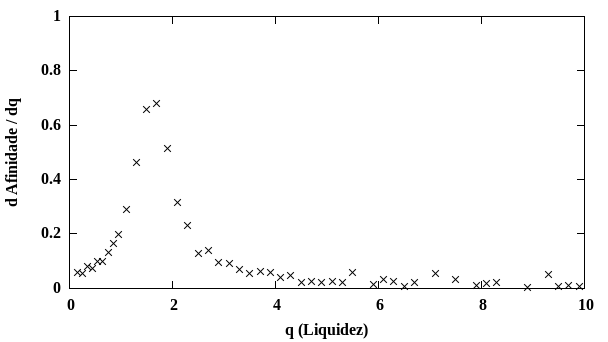
\includegraphics[width=.7\linewidth]{L50-derivada.png}
    \caption{Gráfico da derivada da afinidade em função da liquidez $q$ para $L=50$. O máximo dos pontos obtidos tem o valor $0.68122$ com maximizador $q=1.7$.}
    \label{fig:L50-derivada}
  \end{figure}

  \begin{figure}[h]
    \centering
    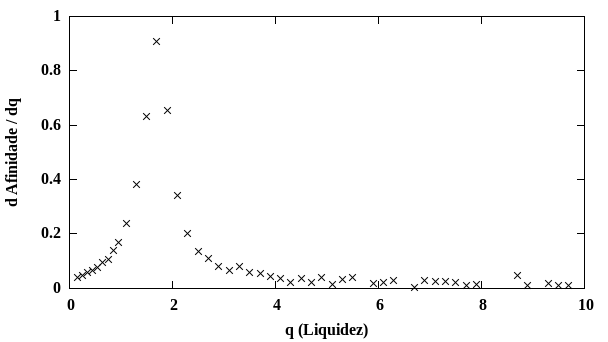
\includegraphics[width=.7\linewidth]{L100-derivada.png}
    \caption{Gráfico da derivada da afinidade em função da liquidez $q$ para $L=100$. O máximo dos pontos obtidos tem o valor $0.90989$ com maximizador $q=1.7$.}
    \label{fig:L100-derivada}
  \end{figure}

  \begin{figure}[h]
    \centering
    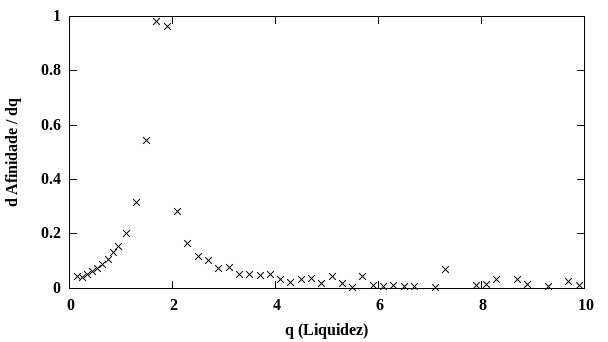
\includegraphics[width=.7\linewidth]{L250-derivada.png}
    \caption{Gráfico da derivada da afinidade em função da liquidez $q$ para $L=250$. O máximo dos pontos obtidos tem o valor $0.98206$ com maximizador $q=1.7$.}
    \label{fig:L250-derivada}
  \end{figure}

  A leitura do artigo ``Stochastic Cellular Automata Model for Stock Market Dynamics'' dos autores M. Bartolozzi e A. W. Thomas;

  Para os próximos dias, estas serão as tarefas realizadas:
  \begin{enumerate}
    \item Escrita de um programa que utiliza o método dos mínimos quadrados para a obtenção da afinidade para os dados com $L=500$.
    \item Explicação do porquê de o limiar intrínseco a cada célula ser considerado como um determinador do momento certo para vender ou comprar;
    \item Simulação para as combinações com $L = 1000$ e $q\in\{$ 
    $0.2,$ $0.4,$ $0.6,$ $0.8,$ $1,$ 
    $1.2,$ $1.4,$ $1.6,$ $1.8,$ $2,$ 
    $2.2,$ $2.4,$ $2.6,$ $2.8,$ $3,$
    $3.2,$ $3.4,$ $3.6,$ $3.8,$ $4,$
    $4.2,$ $4.4,$ $4.6,$ $4.8,$ $5,$
    $5.2,$ $5.4,$ $5.6,$ $5.8,$ $6,$
    $6.2,$ $6.4,$ $6.6,$ $6.8,$ $7,$ 
    $7.2,$ $7.4,$ $7.6,$ $7.8,$ $8,$
    $8.2,$ $8.4,$ $8.6,$ $8.8,$ $9,$ 
    $9.2,$ $9.4,$ $9.6,$ $9.8,$ $10\}$, pois é nessa região que estão os dados que caracterizam a sigmóide;
		\item Pesquisa sobre como a volatilidade de mercado influencia na aglomeração dos agentes;
	\end{enumerate}

\end{document}
